\documentclass{article}


% if you need to pass options to natbib, use, e.g.:
%     \PassOptionsToPackage{numbers, compress}{natbib}
% before loading neurips_2025



\usepackage{amsmath,amsfonts,bm}

\newcommand{\figleft}{{\em (Left)}}
\newcommand{\figcenter}{{\em (Center)}}
\newcommand{\figright}{{\em (Right)}}
\newcommand{\figtop}{{\em (Top)}}
\newcommand{\figbottom}{{\em (Bottom)}}
\newcommand{\captiona}{{\em (a)}}
\newcommand{\captionb}{{\em (b)}}
\newcommand{\captionc}{{\em (c)}}
\newcommand{\captiond}{{\em (d)}}

\newcommand{\newterm}[1]{{\bf #1}}


\def\figref#1{figure~\ref{#1}}
\def\Figref#1{Figure~\ref{#1}}
\def\twofigref#1#2{figures \ref{#1} and \ref{#2}}
\def\quadfigref#1#2#3#4{figures \ref{#1}, \ref{#2}, \ref{#3} and \ref{#4}}
\def\secref#1{section~\ref{#1}}
\def\Secref#1{Section~\ref{#1}}
\def\twosecrefs#1#2{sections \ref{#1} and \ref{#2}}
\def\secrefs#1#2#3{sections \ref{#1}, \ref{#2} and \ref{#3}}
\def\eqref#1{equation~\ref{#1}}
\def\Eqref#1{Equation~\ref{#1}}
\def\plaineqref#1{\ref{#1}}
\def\chapref#1{chapter~\ref{#1}}
\def\Chapref#1{Chapter~\ref{#1}}
\def\rangechapref#1#2{chapters\ref{#1}--\ref{#2}}
\def\algref#1{algorithm~\ref{#1}}
\def\Algref#1{Algorithm~\ref{#1}}
\def\twoalgref#1#2{algorithms \ref{#1} and \ref{#2}}
\def\Twoalgref#1#2{Algorithms \ref{#1} and \ref{#2}}
\def\partref#1{part~\ref{#1}}
\def\Partref#1{Part~\ref{#1}}
\def\twopartref#1#2{parts \ref{#1} and \ref{#2}}

\def\ceil#1{\lceil #1 \rceil}
\def\floor#1{\lfloor #1 \rfloor}
\def\1{\bm{1}}
\newcommand{\train}{\mathcal{D}}
\newcommand{\valid}{\mathcal{D_{\mathrm{valid}}}}
\newcommand{\test}{\mathcal{D_{\mathrm{test}}}}

\def\eps{{\epsilon}}


\def\reta{{\textnormal{$\eta$}}}
\def\ra{{\textnormal{a}}}
\def\rb{{\textnormal{b}}}
\def\rc{{\textnormal{c}}}
\def\rd{{\textnormal{d}}}
\def\re{{\textnormal{e}}}
\def\rf{{\textnormal{f}}}
\def\rg{{\textnormal{g}}}
\def\rh{{\textnormal{h}}}
\def\ri{{\textnormal{i}}}
\def\rj{{\textnormal{j}}}
\def\rk{{\textnormal{k}}}
\def\rl{{\textnormal{l}}}
\def\rn{{\textnormal{n}}}
\def\ro{{\textnormal{o}}}
\def\rp{{\textnormal{p}}}
\def\rq{{\textnormal{q}}}
\def\rr{{\textnormal{r}}}
\def\rs{{\textnormal{s}}}
\def\rt{{\textnormal{t}}}
\def\ru{{\textnormal{u}}}
\def\rv{{\textnormal{v}}}
\def\rw{{\textnormal{w}}}
\def\rx{{\textnormal{x}}}
\def\ry{{\textnormal{y}}}
\def\rz{{\textnormal{z}}}

\def\rvepsilon{{\mathbf{\epsilon}}}
\def\rvtheta{{\mathbf{\theta}}}
\def\rva{{\mathbf{a}}}
\def\rvb{{\mathbf{b}}}
\def\rvc{{\mathbf{c}}}
\def\rvd{{\mathbf{d}}}
\def\rve{{\mathbf{e}}}
\def\rvf{{\mathbf{f}}}
\def\rvg{{\mathbf{g}}}
\def\rvh{{\mathbf{h}}}
\def\rvu{{\mathbf{i}}}
\def\rvj{{\mathbf{j}}}
\def\rvk{{\mathbf{k}}}
\def\rvl{{\mathbf{l}}}
\def\rvm{{\mathbf{m}}}
\def\rvn{{\mathbf{n}}}
\def\rvo{{\mathbf{o}}}
\def\rvp{{\mathbf{p}}}
\def\rvq{{\mathbf{q}}}
\def\rvr{{\mathbf{r}}}
\def\rvs{{\mathbf{s}}}
\def\rvt{{\mathbf{t}}}
\def\rvu{{\mathbf{u}}}
\def\rvv{{\mathbf{v}}}
\def\rvw{{\mathbf{w}}}
\def\rvx{{\mathbf{x}}}
\def\rvy{{\mathbf{y}}}
\def\rvz{{\mathbf{z}}}

\def\erva{{\textnormal{a}}}
\def\ervb{{\textnormal{b}}}
\def\ervc{{\textnormal{c}}}
\def\ervd{{\textnormal{d}}}
\def\erve{{\textnormal{e}}}
\def\ervf{{\textnormal{f}}}
\def\ervg{{\textnormal{g}}}
\def\ervh{{\textnormal{h}}}
\def\ervi{{\textnormal{i}}}
\def\ervj{{\textnormal{j}}}
\def\ervk{{\textnormal{k}}}
\def\ervl{{\textnormal{l}}}
\def\ervm{{\textnormal{m}}}
\def\ervn{{\textnormal{n}}}
\def\ervo{{\textnormal{o}}}
\def\ervp{{\textnormal{p}}}
\def\ervq{{\textnormal{q}}}
\def\ervr{{\textnormal{r}}}
\def\ervs{{\textnormal{s}}}
\def\ervt{{\textnormal{t}}}
\def\ervu{{\textnormal{u}}}
\def\ervv{{\textnormal{v}}}
\def\ervw{{\textnormal{w}}}
\def\ervx{{\textnormal{x}}}
\def\ervy{{\textnormal{y}}}
\def\ervz{{\textnormal{z}}}

\def\rmA{{\mathbf{A}}}
\def\rmB{{\mathbf{B}}}
\def\rmC{{\mathbf{C}}}
\def\rmD{{\mathbf{D}}}
\def\rmE{{\mathbf{E}}}
\def\rmF{{\mathbf{F}}}
\def\rmG{{\mathbf{G}}}
\def\rmH{{\mathbf{H}}}
\def\rmI{{\mathbf{I}}}
\def\rmJ{{\mathbf{J}}}
\def\rmK{{\mathbf{K}}}
\def\rmL{{\mathbf{L}}}
\def\rmM{{\mathbf{M}}}
\def\rmN{{\mathbf{N}}}
\def\rmO{{\mathbf{O}}}
\def\rmP{{\mathbf{P}}}
\def\rmQ{{\mathbf{Q}}}
\def\rmR{{\mathbf{R}}}
\def\rmS{{\mathbf{S}}}
\def\rmT{{\mathbf{T}}}
\def\rmU{{\mathbf{U}}}
\def\rmV{{\mathbf{V}}}
\def\rmW{{\mathbf{W}}}
\def\rmX{{\mathbf{X}}}
\def\rmY{{\mathbf{Y}}}
\def\rmZ{{\mathbf{Z}}}

\def\ermA{{\textnormal{A}}}
\def\ermB{{\textnormal{B}}}
\def\ermC{{\textnormal{C}}}
\def\ermD{{\textnormal{D}}}
\def\ermE{{\textnormal{E}}}
\def\ermF{{\textnormal{F}}}
\def\ermG{{\textnormal{G}}}
\def\ermH{{\textnormal{H}}}
\def\ermI{{\textnormal{I}}}
\def\ermJ{{\textnormal{J}}}
\def\ermK{{\textnormal{K}}}
\def\ermL{{\textnormal{L}}}
\def\ermM{{\textnormal{M}}}
\def\ermN{{\textnormal{N}}}
\def\ermO{{\textnormal{O}}}
\def\ermP{{\textnormal{P}}}
\def\ermQ{{\textnormal{Q}}}
\def\ermR{{\textnormal{R}}}
\def\ermS{{\textnormal{S}}}
\def\ermT{{\textnormal{T}}}
\def\ermU{{\textnormal{U}}}
\def\ermV{{\textnormal{V}}}
\def\ermW{{\textnormal{W}}}
\def\ermX{{\textnormal{X}}}
\def\ermY{{\textnormal{Y}}}
\def\ermZ{{\textnormal{Z}}}

\def\vzero{{\bm{0}}}
\def\vone{{\bm{1}}}
\def\vmu{{\bm{\mu}}}
\def\vtheta{{\bm{\theta}}}
\def\va{{\bm{a}}}
\def\vb{{\bm{b}}}
\def\vc{{\bm{c}}}
\def\vd{{\bm{d}}}
\def\ve{{\bm{e}}}
\def\vf{{\bm{f}}}
\def\vg{{\bm{g}}}
\def\vh{{\bm{h}}}
\def\vi{{\bm{i}}}
\def\vj{{\bm{j}}}
\def\vk{{\bm{k}}}
\def\vl{{\bm{l}}}
\def\vm{{\bm{m}}}
\def\vn{{\bm{n}}}
\def\vo{{\bm{o}}}
\def\vp{{\bm{p}}}
\def\vq{{\bm{q}}}
\def\vr{{\bm{r}}}
\def\vs{{\bm{s}}}
\def\vt{{\bm{t}}}
\def\vu{{\bm{u}}}
\def\vv{{\bm{v}}}
\def\vw{{\bm{w}}}
\def\vx{{\bm{x}}}
\def\vy{{\bm{y}}}
\def\vz{{\bm{z}}}

\def\evalpha{{\alpha}}
\def\evbeta{{\beta}}
\def\evepsilon{{\epsilon}}
\def\evlambda{{\lambda}}
\def\evomega{{\omega}}
\def\evmu{{\mu}}
\def\evpsi{{\psi}}
\def\evsigma{{\sigma}}
\def\evtheta{{\theta}}
\def\eva{{a}}
\def\evb{{b}}
\def\evc{{c}}
\def\evd{{d}}
\def\eve{{e}}
\def\evf{{f}}
\def\evg{{g}}
\def\evh{{h}}
\def\evi{{i}}
\def\evj{{j}}
\def\evk{{k}}
\def\evl{{l}}
\def\evm{{m}}
\def\evn{{n}}
\def\evo{{o}}
\def\evp{{p}}
\def\evq{{q}}
\def\evr{{r}}
\def\evs{{s}}
\def\evt{{t}}
\def\evu{{u}}
\def\evv{{v}}
\def\evw{{w}}
\def\evx{{x}}
\def\evy{{y}}
\def\evz{{z}}

\def\mA{{\bm{A}}}
\def\mB{{\bm{B}}}
\def\mC{{\bm{C}}}
\def\mD{{\bm{D}}}
\def\mE{{\bm{E}}}
\def\mF{{\bm{F}}}
\def\mG{{\bm{G}}}
\def\mH{{\bm{H}}}
\def\mI{{\bm{I}}}
\def\mJ{{\bm{J}}}
\def\mK{{\bm{K}}}
\def\mL{{\bm{L}}}
\def\mM{{\bm{M}}}
\def\mN{{\bm{N}}}
\def\mO{{\bm{O}}}
\def\mP{{\bm{P}}}
\def\mQ{{\bm{Q}}}
\def\mR{{\bm{R}}}
\def\mS{{\bm{S}}}
\def\mT{{\bm{T}}}
\def\mU{{\bm{U}}}
\def\mV{{\bm{V}}}
\def\mW{{\bm{W}}}
\def\mX{{\bm{X}}}
\def\mY{{\bm{Y}}}
\def\mZ{{\bm{Z}}}
\def\mBeta{{\bm{\beta}}}
\def\mPhi{{\bm{\Phi}}}
\def\mLambda{{\bm{\Lambda}}}
\def\mSigma{{\bm{\Sigma}}}

\DeclareMathAlphabet{\mathsfit}{\encodingdefault}{\sfdefault}{m}{sl}
\SetMathAlphabet{\mathsfit}{bold}{\encodingdefault}{\sfdefault}{bx}{n}
\newcommand{\tens}[1]{\bm{\mathsfit{#1}}}
\def\tA{{\tens{A}}}
\def\tB{{\tens{B}}}
\def\tC{{\tens{C}}}
\def\tD{{\tens{D}}}
\def\tE{{\tens{E}}}
\def\tF{{\tens{F}}}
\def\tG{{\tens{G}}}
\def\tH{{\tens{H}}}
\def\tI{{\tens{I}}}
\def\tJ{{\tens{J}}}
\def\tK{{\tens{K}}}
\def\tL{{\tens{L}}}
\def\tM{{\tens{M}}}
\def\tN{{\tens{N}}}
\def\tO{{\tens{O}}}
\def\tP{{\tens{P}}}
\def\tQ{{\tens{Q}}}
\def\tR{{\tens{R}}}
\def\tS{{\tens{S}}}
\def\tT{{\tens{T}}}
\def\tU{{\tens{U}}}
\def\tV{{\tens{V}}}
\def\tW{{\tens{W}}}
\def\tX{{\tens{X}}}
\def\tY{{\tens{Y}}}
\def\tZ{{\tens{Z}}}


\def\gA{{\mathcal{A}}}
\def\gB{{\mathcal{B}}}
\def\gC{{\mathcal{C}}}
\def\gD{{\mathcal{D}}}
\def\gE{{\mathcal{E}}}
\def\gF{{\mathcal{F}}}
\def\gG{{\mathcal{G}}}
\def\gH{{\mathcal{H}}}
\def\gI{{\mathcal{I}}}
\def\gJ{{\mathcal{J}}}
\def\gK{{\mathcal{K}}}
\def\gL{{\mathcal{L}}}
\def\gM{{\mathcal{M}}}
\def\gN{{\mathcal{N}}}
\def\gO{{\mathcal{O}}}
\def\gP{{\mathcal{P}}}
\def\gQ{{\mathcal{Q}}}
\def\gR{{\mathcal{R}}}
\def\gS{{\mathcal{S}}}
\def\gT{{\mathcal{T}}}
\def\gU{{\mathcal{U}}}
\def\gV{{\mathcal{V}}}
\def\gW{{\mathcal{W}}}
\def\gX{{\mathcal{X}}}
\def\gY{{\mathcal{Y}}}
\def\gZ{{\mathcal{Z}}}

\def\sA{{\mathbb{A}}}
\def\sB{{\mathbb{B}}}
\def\sC{{\mathbb{C}}}
\def\sD{{\mathbb{D}}}
\def\sF{{\mathbb{F}}}
\def\sG{{\mathbb{G}}}
\def\sH{{\mathbb{H}}}
\def\sI{{\mathbb{I}}}
\def\sJ{{\mathbb{J}}}
\def\sK{{\mathbb{K}}}
\def\sL{{\mathbb{L}}}
\def\sM{{\mathbb{M}}}
\def\sN{{\mathbb{N}}}
\def\sO{{\mathbb{O}}}
\def\sP{{\mathbb{P}}}
\def\sQ{{\mathbb{Q}}}
\def\sR{{\mathbb{R}}}
\def\sS{{\mathbb{S}}}
\def\sT{{\mathbb{T}}}
\def\sU{{\mathbb{U}}}
\def\sV{{\mathbb{V}}}
\def\sW{{\mathbb{W}}}
\def\sX{{\mathbb{X}}}
\def\sY{{\mathbb{Y}}}
\def\sZ{{\mathbb{Z}}}

\def\emLambda{{\Lambda}}
\def\emA{{A}}
\def\emB{{B}}
\def\emC{{C}}
\def\emD{{D}}
\def\emE{{E}}
\def\emF{{F}}
\def\emG{{G}}
\def\emH{{H}}
\def\emI{{I}}
\def\emJ{{J}}
\def\emK{{K}}
\def\emL{{L}}
\def\emM{{M}}
\def\emN{{N}}
\def\emO{{O}}
\def\emP{{P}}
\def\emQ{{Q}}
\def\emR{{R}}
\def\emS{{S}}
\def\emT{{T}}
\def\emU{{U}}
\def\emV{{V}}
\def\emW{{W}}
\def\emX{{X}}
\def\emY{{Y}}
\def\emZ{{Z}}
\def\emSigma{{\Sigma}}

\newcommand{\etens}[1]{\mathsfit{#1}}
\def\etLambda{{\etens{\Lambda}}}
\def\etA{{\etens{A}}}
\def\etB{{\etens{B}}}
\def\etC{{\etens{C}}}
\def\etD{{\etens{D}}}
\def\etE{{\etens{E}}}
\def\etF{{\etens{F}}}
\def\etG{{\etens{G}}}
\def\etH{{\etens{H}}}
\def\etI{{\etens{I}}}
\def\etJ{{\etens{J}}}
\def\etK{{\etens{K}}}
\def\etL{{\etens{L}}}
\def\etM{{\etens{M}}}
\def\etN{{\etens{N}}}
\def\etO{{\etens{O}}}
\def\etP{{\etens{P}}}
\def\etQ{{\etens{Q}}}
\def\etR{{\etens{R}}}
\def\etS{{\etens{S}}}
\def\etT{{\etens{T}}}
\def\etU{{\etens{U}}}
\def\etV{{\etens{V}}}
\def\etW{{\etens{W}}}
\def\etX{{\etens{X}}}
\def\etY{{\etens{Y}}}
\def\etZ{{\etens{Z}}}

\newcommand{\pdata}{p_{\rm{data}}}
\newcommand{\ptrain}{\hat{p}_{\rm{data}}}
\newcommand{\Ptrain}{\hat{P}_{\rm{data}}}
\newcommand{\pmodel}{p_{\rm{model}}}
\newcommand{\Pmodel}{P_{\rm{model}}}
\newcommand{\ptildemodel}{\tilde{p}_{\rm{model}}}
\newcommand{\pencode}{p_{\rm{encoder}}}
\newcommand{\pdecode}{p_{\rm{decoder}}}
\newcommand{\precons}{p_{\rm{reconstruct}}}

\newcommand{\laplace}{\mathrm{Laplace}} %

\newcommand{\E}{\mathbb{E}}
\newcommand{\Ls}{\mathcal{L}}
\newcommand{\R}{\mathbb{R}}
\newcommand{\emp}{\tilde{p}}
\newcommand{\lr}{\alpha}
\newcommand{\reg}{\lambda}
\newcommand{\rect}{\mathrm{rectifier}}
\newcommand{\softmax}{\mathrm{softmax}}
\newcommand{\sigmoid}{\sigma}
\newcommand{\softplus}{\zeta}
\newcommand{\KL}{D_{\mathrm{KL}}}
\newcommand{\Var}{\mathrm{Var}}
\newcommand{\standarderror}{\mathrm{SE}}
\newcommand{\Cov}{\mathrm{Cov}}
\newcommand{\normlzero}{L^0}
\newcommand{\normlone}{L^1}
\newcommand{\normltwo}{L^2}
\newcommand{\normlp}{L^p}
\newcommand{\normmax}{L^\infty}

\newcommand{\parents}{Pa} %

\DeclareMathOperator*{\argmax}{arg\,max}
\DeclareMathOperator*{\argmin}{arg\,min}

\DeclareMathOperator{\sign}{sign}
\DeclareMathOperator{\Tr}{Tr}
\let\ab\allowbreak
% ready for submission
\usepackage{neurips_2025}
\usepackage{graphicx} % Required for \resizebox
\usepackage{xspace}
\newcommand{\mmdit}{\textit{MM-DiT}\xspace}
% to compile a preprint version, e.g., for submission to arXiv, add add the
% [preprint] option:
%     \usepackage[preprint]{neurips_2025}


% to compile a camera-ready version, add the [final] option, e.g.:
%     \usepackage[final]{neurips_2025}


% to avoid loading the natbib package, add option nonatbib:
%    \usepackage[nonatbib]{neurips_2025}


\usepackage[utf8]{inputenc} % allow utf-8 input
\usepackage[T1]{fontenc}    % use 8-bit T1 fonts
\usepackage{hyperref}       % hyperlinks
\usepackage{url}            % simple URL typesetting
\usepackage{booktabs}       % professional-quality tables
\usepackage{amsfonts}       % blackboard math symbols
\usepackage{nicefrac}       % compact symbols for 1/2, etc.
\usepackage{microtype}      % microtypography
\usepackage{xcolor}         % colors
\usepackage{amsmath}

\title{CannyEdit: Regional Image Editing with Canny Edge Guidance in Pretrained Diffusion Models}


% The \author macro works with any number of authors. There are two commands
% used to separate the names and addresses of multiple authors: \And and \AND.
%
% Using \And between authors leaves it to LaTeX to determine where to break the
% lines. Using \AND forces a line break at that point. So, if LaTeX puts 3 of 4
% authors names on the first line, and the last on the second line, try using
% \AND instead of \And before the third author name.


\author{%
  David S.~Hippocampus\thanks{Use footnote for providing further information
    about author (webpage, alternative address)---\emph{not} for acknowledging
    funding agencies.} \\
  Department of Computer Science\\
  Cranberry-Lemon University\\
  Pittsburgh, PA 15213 \\
  \texttt{hippo@cs.cranberry-lemon.edu} \\
  % examples of more authors
  % \And
  % Coauthor \\
  % Affiliation \\
  % Address \\
  % \texttt{email} \\
  % \AND
  % Coauthor \\
  % Affiliation \\
  % Address \\
  % \texttt{email} \\
  % \And
  % Coauthor \\
  % Affiliation \\
  % Address \\
  % \texttt{email} \\
  % \And
  % Coauthor \\
  % Affiliation \\
  % Address \\
  % \texttt{email} \\
}




\begin{document}


\maketitle


\begin{abstract}
  The abstract paragraph should be indented \nicefrac{1}{2}~inch (3~picas) on
  both the left- and right-hand margins. Use 10~point type, with a vertical
  spacing (leading) of 11~points.  The word \textbf{Abstract} must be centered,
  bold, and in point size 12. Two line spaces precede the abstract. The abstract
  must be limited to one paragraph.
\end{abstract}


\begin{figure}[h!]
    \centering
    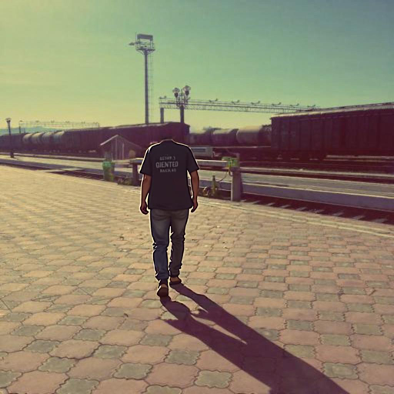
\includegraphics[width=0.5\linewidth]{image1.png}
    \caption{An example to showcase that CannyEdit can be applied to different tasks}
    \label{fig1}
\end{figure}


\section{Introduction}

%, beginning with Stable Diffusion \citep{rombach2022high} and DALL$\cdot$E 3 \citep{betker2023improving}, which utilize UNet and diffusion models (DMs) \citep{rombach2022high}. More recent developments include the FLUX \citep{blackforest2024flux} and SD3 model \citep{esser2024scaling}, which adopt the diffusion transformer (DiT) architecture \citep{peebles2023scalable} and rectified flow models \citep{liu2022flow, lipman2022flow}. 

Recent advances in text-to-image (T2I) models have demonstrated significant progress \citep{rombach2022high,betker2023improving,chen2023pixart,esser2024scaling,blackforest2024flux}. Building on these advancements, many downstream applications have emerged, leveraging the improved quality, efficiency, and versatility of these models.  In this paper, we focus on one of the most challenging applications: regional image editing. This task involves making specific edits (e.g., object adding, replacement or removal, see examples in Figure \ref{fig1}) to given areas of a generated or real-world image while keeping the rest of the image unchanged. It is effectively a conditioned T2I generation task, where the additional condition is the existing content in other parts of the image. The key challenge is to ensure that the edits in the specific area not only match the input text but also blend coherently with the surrounding content. Ideally, if the editing is seamless, it should be difficult for viewers to discern the edited region or notice that the image has been modified by a model. 



A straightforward approach to regional editing involves collecting paired training data (before and after editing), along with corresponding text prompts, to train models for editing \citep{brooks2023instructpix2pix, zhang2023magicbrush, wasserman2024paint, li2024brushedit, hui2024hq, wei2024omniedit}. However, these methods often struggle to generalize beyond their training distribution—particularly in cases requiring realistic interactions, such as inserting people into complex scenes. This limitation is largely attributed to the lack of diverse, high-quality training data capturing such interactions.

Consequently, by tapping into foundation T2I models’ ability to capture realistic object interactions from large-scale datasets, another line of research explores using these foundation models for regional editing in a training-free manner. While these methods were initially developed using UNet-based diffusion models \citep{hertz2022prompt, cao2023masactrl, tumanyan2023plug}, recent work has shifted to leveraging more advanced rectified-flow-based diffusion transformers (DiTs) \citep{rout2024semantic, wang2024taming, deng2024fireflow, tewel2025addit, zhu2025kv}, predominantly designed based on the leading open-source DiT model, FLUX.1-dev \citep{blackforest2024flux}.


%These newer DiT-based methods (\citep{rout2024semantic, wang2024taming, deng2024fireflow, tewel2025addit, zhu2025kv}) have demonstrated improved editing performance and greater flexibility compared to earlier UNet-based approaches, benefiting from the stronger generative power and the modular architecture of DiTs.


In this study, we further investigate the use of advanced DiTs for regional editing. Existing training-free methods typically follow a two-stage attention-based editing pipeline: (1) Inversion: the source image is inverted into the DiT’s latent space to extract attention features at each denoising step; (2) Source-attention injection: these features are injected into the attention computation during the generation of the target image. However, challenges persist: (1) Methods such as Add-it \citep{tewel2025addit}, RF-Inversion-Edit \citep{rout2024semantic}, and FireFlow-Edit \citep{deng2024fireflow} struggle to balance local edits with background fidelity, often failing with major layout changes (e.g., adding a human subject results in undersized or failed objects); (2) KV-Edit \citep{zhu2025kv} supports larger layout changes by using a mask to decouple the background and edit regions, but its decoupled attention mechanism disrupts cross-region coherence, which could result in unrealistic interactions between edited regions and the original context, especially in the adding task. These challenges underscore the difficulty of maintaining both editability and background fidelity using source-image attention features.
%produces unrealistic interactions due to its 

%(1) \textbf{Inversion}: the source image is inverted into the DiT’s latent space to extract attention features at each denoising step; (2) \textbf{Source-attention injection}: these attention features from the inversion are injected into the attention computation during the generation of the target image. However, challenges remain for these methods: (1) Methods like Add-it \citep{tewel2025addit}, RF-Inversion-Edit \citep{rout2024semantic}, RF-Solver-Edit \citep{wang2024taming}, and FireFlow-Edit \citep{deng2024fireflow} struggle to balance local editability with background fidelity. While using attention features from the source image preserves background fidelity, these methods falter with substantial layout changes (e.g., adding a human subject often leads to undersized or failed object generation). (2) KV-Edit \citep{zhu2025kv} supports larger layout changes but often produces unrealistic interactions between edited regions and the original context. The core issue lies in KV-Edit’s decoupled attention mechanism, where keys and values are sourced differently (background from the inverted source vs. edits from current denoising), disrupting cross-region coherence. These challenges highlight the intrinsic difficulty in balancing local editability with background fidelity when integrating source-image attention features into the attention mechanism. 




Observing the challenges, we propose a novel approach that departs from conventional attention-based methods by leveraging Canny edge guidance for editing. The Canny edge map \citep{Canny1986computational} captures the general layout information of the image, representing the spatial arrangement of objects in the scene through their outlines. The use of Canny edge guidance has been widely explored in generating the whole image, as exemplified by ControlNet \citep{zhang2023adding}. Canny ControlNet is a plug-and-play module for foundation T2I models, incorporating copies of the T2I model's denoising blocks to process input Canny edge maps. During inference, ControlNet's outputs are directly added into the corresponding blocks of the foundation T2I model without altering the foundation model's text-image attention computation process, enabling image generation that is aligned with text prompts and guided by Canny structural information.


Compared to Canny-guided image generation, Canny-guided regional image editing has been little explored. The reasons why Canny guidance with foundation T2I models could be useful for regional editing include the following:


First, the Canny ControlNet allows control over the general image layout. By using the same Canny edge map with different text prompts, edits can be made while preserving the layout. For example, Figure \ref{fig2}(a) demonstrates that FLUX.1-dev \citep{blackforest2024flux}, combined with the Canny ControlNet \citep{xlabsai2025fluxcontrolnet}, consistently places different subjects (a, a.1, a.2) in the same location based on the given edge map when different text prompts are provided.

Second, selectively masking Canny control allows for the local editability while preserving the layout of other areas. Outputs from the Canny ControlNet are optional for T2I generation models—when provided, generation combines text prompts and structural Canny information; otherwise, it relies solely on text prompts. We found that the T2I model is also capable of handling partial outputs from ControlNet, where the ControlNet outputs for specific regions are set to zero before being added to the T2I model, allowing layout flexibility in those regions while maintaining the layout elsewhere. For instance, adding a person to a dining room image introduces layout challenges where full Canny control struggles with positioning (Figure \ref{fig2}(b.1)). However, by adding partially masked ControlNet outputs, where features in the targeted region (black area in (b.Canny mask)) is zeroed out, to the T2I model, the new subject can be successfully placed in the intended location, blending seamlessly with the surrounding image context (Figure \ref{fig2}(b.2)).



Leveraging the flexibility of the Canny control, this work proposes a regional editing method named \textbf{\textit{CannyEdit}}, which applies Canny guidance to image editing. Central to the method is the \textit{selective Canny masking} mechanism that suppresses edge guidance in user-specified regions, enabling localized edits while preserving the structural image layout elsewhere. 

To further maintain background fidelity, we apply the image inversion process on the source image, which integrates a Canny ControlNet to record the Canny control signals of the source image. These signals are selectively masked and injected into the T2I denoising steps during the generation of the edited image

%To further maintain background fidelity, we apply the image inversion process on the source image, which integrates a Canny ControlNet to record the Canny control signals of the source image. These signals are selectively masked and injected into the T2I denoising steps during the generation of the edited image. 

We further combine regional text prompts with attention masks for granular control, allowing targeted textual control in specific areas without compromising global coherence. By unifying these techniques, CannyEdit emerges as a versatile and powerful regional image editing framework, capable of handling a wide range of image editing tasks.




In summary, we make the following key contributions in this paper:
\vspace{-1mm}
\begin{itemize}
    %\item To the best of our knowledge, our proposed CannyEdit is the first Canny-guided regional image editing method, incorporating the selective Canny control to enable both the local editability and background fidelity;
    \item To the best of our knowledge,  our proposed CannyEdit CannyEdit is the first Canny-guided regional image editing framework built on foundation T2I models. We introduce a selective Canny masking mechanism that flexibly suppresses edge guidance in user-specified regions, enabling precise local edits while preserving the structural layout. %and background fidelity of unedited areas through image inversion with integrated Canny ControlNet signals.
    \item CannyEdit is highly flexible, being able to apply different regional image editing tasks, including object transfer, adding, replacement, removal; context change and object personalization;
    \item We show that CannyEdit maintains high level of image quality, background preservation and text alignment on the PIE-Bench \citep{brooks2023instructpix2pix}. Since there is lack of benchmark that evaluates the editing seamlessness performance in real-world image editing, we construct a ``real-world editing seamlessness'' benchmark and conduct user study to evaluate if the users can discern the edited region or notice that the image has been modified by a model. CannyEdit shows significantly improved seamlessness compared to previous training-based and training-free methods \textcolor{red}{[Need exact numbers]}. 
\end{itemize}


% 1. 是否生成
% 2. better edit
% 3. 给原图跟生成图,问哪一张是生成图
% 4. 给生成图,问哪一块是生成的

%==================================
% Two trade-offs:

% Local editability vs. Background consistency

% Local controllability vs. Global affordance

% To make a good balance on the two trade-offs, we propose an editing method based on the Canny layout control via ControlNet. To maintain the background consistency, we apply the Canny control on the background to maintain the layout of the background unchanged.  To allow the local editability, the related region in the Canny control is revised to be zero. In the later denoising steps, blending operation is applied to ensure the visual details of the background is unchanged on top of the maintained layout preserved by the ControlNet. Note that the unchanged background layout also makes sure that the generated object is semantically fitted with the original environment well if the objects can be generated.

% To enable a good balance of local controllability and global affordance, we apply regional control with attention mask where local editing text prompts is cross-attended with edited image region, and a context prompt which describes the image after editing is cross-attended  with whole image.

%==================================



%  4. Our Canny control-based method: \textcolor{red}{\textbf{why Canny? why Canny controlnet?}}

% trade-offs: local editability vs. background fidelity; affordance.
% not to do attention sharing








\begin{figure}[t]
    \centering
    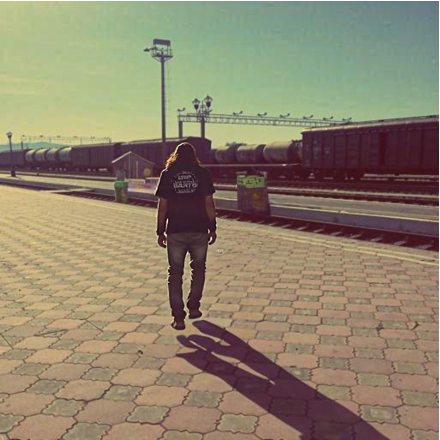
\includegraphics[width=0.5\linewidth]{image2.png}
    \caption{Group Space-Progress2504-paperfigures-figure2.png. (a, a.1, a.2) are generated based on the same Canny.}
    \label{fig2}
\end{figure}


\section{Related work}
\subsection{Training-based regional editing methods}

A significant number of studies focus on training-based methods for image editing. Although it is beneficial to teach model to learn to follow instructions, it is very expensive to collect high-quality image editing data. Therefore, many works propose to use synthetic data. For example, InstructPix2Pix \citep{brooks2023instructpix2pix} uses a language model (GPT-3) and a text-to-image model (Stable Diffusion) to generate a synthetic dataset of image editing examples. Similarly, HQ-Edit \citep{hui2024hq} uses GPT-4V and DALL-E 3. These methods, which reply on synthetic data, may not capture all real-world nuances, potentially limiting performance on complex edits.

A different line of work collects real-world images and invites humans to manually annotate data or use task specialists (pre-trained image-editing models) to generate target images. MagicBrush \citep{zhang2023magicbrush} consists of 10K manually annotated real image editing triplets (source image,
instruction, target image), but it is very difficult to scale it up.  PIPE (Paint by Inpaint Edit) \citep{wasserman2024paint} contains approximately 1 million image pairs, where objects are removed from source images using SD-inpainting model \footnote{https://huggingface.co/runwayml/stable-diffusion-inpainting}, but it is only focused on object adding task. OmniEdit \citep{wei2024omniedit} is a generalist model trained on over 1 million pairs covering diverse editing skills, leveraging the supervision from seven specialist models. The computational costs of constructing the datasets and training the model are significant, as they scale with the complexity of the models and the volume of data being processed. 

The challenge of dataset scalability limits the generalization performance of training-based methods. We argue that training-free methods are better alternatives. Not only because they are computaionally e


\subsection{Training-free regional editing methods}

UNet-based: P2P;
DiT-based: how to do inversion, how to do source-attention injection.

\subsection{Controllability in T2I generation}

 To enhance the controllability of the T2I generation, efforts have been made to make the generation based on extra conditional control, like the Canny control, depth control in ControlNet \citep{zhang2023adding}, layout control in \citet{feng2024ranni,yang2024mastering} and the subject control in \citet{ye2023ip,wang2024instantid}. 

\section{Canny-guided image editing}
\subsection{Preliminaries}
%\subsubsection{MM-DiTs and Canny ControlNet}
% \subsubsection{Canny ControlNet}
% \subsubsection{Inversion methods for DiTs}

% \subsection{ControlNet in inversion}

Modern Diffusion Transformers (DiTs) models, such as SD3 \citep{esser2024scaling} and FLUX \citep{blackforest2024flux}, process concatenated sequences of textual-prompt and image-patch tokens through unified multi-modal self-attention blocks (\mmdit blocks). Specifically, FLUX has two types of attention blocks: \textbf{Multi-stream}  blocks which use separate projection matrices ($\mW_K, \mW_V, \mW_Q$) for text and image tokens, and \textbf{Single-stream} blocks where the same projection matrices are used for both. Both block types compute attention on the concatenated tokens to get the hidden state $h$ as follows:
\begin{equation}
    A = \textit{softmax}([Q_{p}, Q_{img}] [K_{p}, K_{img}]^\top / \sqrt{d_k}),\quad h = A \cdot [V_{p}, V_{img}],\quad h_{img} =  A_{img} \cdot [V_{p}, V_{img}] \label{eq:flux_attention}
\end{equation}
where $Q_{p}$, $Q_{img}$ are the textual-prompt and the image-patch queries, respectively, and $A_{img}$  denotes the rows of $A$ corresponding to the image-patch tokens. The same applies to $K$ and $V$.
Notably, FLUX is composed of a series of Multi-stream blocks followed by a series of Single-stream blocks. 

In the self-attention blocks of the FLUX model:
\begin{equation}
Q_{img}^{flux}=\mW_Q^{flux}(\mathbf{z}_{t_{i}}), K_{img}^{flux}=\mW_K^{flux}(\mathbf{z}_{t_{i}}), V_{img}^{flux}=\mW_V^{flux}(\mathbf{z}_{t_{i}})
\label{eq:qkv_flux}
\end{equation}

In the self-attention blocks of the Canny ControlNet:

\begin{equation}
Q_{img}^{ca}=\mW_Q^{ca}(\mathbf{z}_{t_{i}}+\mathcal{F}(Canny)), K_{img}^{ca}=\mW_K^{ca}(\mathbf{z}_{t_{i}}+\mathcal{F}(Canny)), V_{img}^{ca}=\mW_V^{ca}(\mathbf{z}_{t_{i}}+\mathcal{F}(Canny)),
\label{eq:qkv_controlnet}
\end{equation}

where $Canny$ is the input Canny edge map, and $\mathcal{F}(\cdot)$ denotes the operations that map the Canny edge map to a latent representation of the same size as $\mathbf{z}_{t_{i}}$, including a convolutional layer and an MLP layer. 
Substituting the Queries, Keys, Values in Equation (\ref{eq:qkv_flux}) and (\ref{eq:qkv_controlnet}) into Equation (\ref{eq:flux_attention}) respectively, we can get $h^{flux}_{img}$ and $h^{ca}_{img}$.

Note that the Canny ControlNet only includes copies of two Multi-stream blocks but not the Single-stream blocks. At each Multi-stream block with index \( i \), the image hidden state \( h^{\text{flux}}_{\text{img}}[i] \) from the Flux model is updated by adding the corresponding ControlNet hidden state, following:

\[
h^{\text{flux}}_{\text{img}}[i] \leftarrow h^{\text{flux}}_{\text{img}}[i] + \beta\cdot h^{ca}_{\text{img}}[i \bmod 2],
\]

where \( i \bmod 2 \) selects between the two ControlNet hidden states cyclically according to the block index \( i \), where $\beta$ is a hyperparameter that decides the strength of Canny control.

% copies of the T2I model's denoising blocks 

%FLUX is composed of a series of Multi-stream blocks followed by a series of Single-stream blocks. 




%Taking Rectified Flow~\cite{liu2022rectified,rectflow} as an example, based on \cref{eq:4}, 

We can derive the discretized implementation of inversion and denoising. The model takes the original image $\mathbf{x}_{t_0}$ and Gaussian noise $\mathbf{x}_{t_N}\in\mathcal{N}(0,\boldsymbol{I})$ as path endpoints. Given discrete timesteps $t=\{t_{N},...,t_{0}\}$, the model predictions $\boldsymbol{v}_\theta(C,\mathbf{x}_{t_i},t_i),i\in\{N,\cdots,1\}$, where $\mathbf{x}_{t_i}$ and $\mathbf{z}_{t_i}$ denote intermediate states in inversion and denoising respectively, as described by the following equations:
\begin{equation}
\mathbf{x}_{t_{i}}=\mathbf{x}_{t_{i-1}}+(t_i-t_{i-1})\boldsymbol{v}_\theta(C,\mathbf{x}_{t_i},t_i)
\end{equation}
\begin{equation}
\mathbf{z}_{t_{i-1}}=\mathbf{z}_{t_i}+(t_{i-1}-t_i)\boldsymbol{v}_\theta(C,\mathbf{z}_{t_i},t_i) 
\end{equation}
Ideally, $\mathbf{z}_{t_0}$ should be identity with $\mathbf{x}_{t_0}$ when directly reconstructed from $\mathbf{x}_{t_N}$. However, due to discretization and causality in the inversion process, we can only estimate using $\boldsymbol{v}_\theta(C,\mathbf{X}_{t_{t-1}},t_{t-1}) \approx \boldsymbol{v}_\theta(C,\mathbf{X}_{t_i},t_i)$, introducing cumulative errors. 

%\cref{fig:skip} shows that with a fixed number of timesteps $N$, error accumulation increases as inversion timesteps approach $t_{N}$, preventing accurate reconstruction.





\subsection{Selective Canny control}
%regional Canny relaxation

\subsection{Incorporation of regional control in image editing}


\subsection{Application to different regional editing tasks}

\subsubsection{Object transfer, replacement and context change}

%\subsection{Object transfer with full Canny control}

%\textcolor{red}{Examples (Figure \ref{fig1}) to showcase that direct regional control cannot make edits. However, selective Canny masking can allow the local editability.}


%\subsection{Regional image editing with selective Canny control}

\subsubsection{Object adding with mask refinement}

% Preservation of original information in edited region
% Mask acquisition of the generated objects
% Synthetic Canny
% Cyclical blending 
%To allow the generation of collateral objects but maintain the background mainly unchanged, we do the cyclical blending with partial blending on the background region with the inversion latent.

\subsubsection{Object removal with regional CFG}


\subsubsection{Personalization with copy-paste synthesis}
%\subsection{Extension to different tasks}


\begin{table}[h!]
\centering
\caption{Technical Summary}
 \vskip 1em
\resizebox{\textwidth}{!}{%
\begin{tabular}{l l l l l}
\toprule
Task & Definition & Inputs & Canny Guidance & Regional Control\\
\midrule
Object Transfer & Replace an object with another, & source prompt, target prompt, local prompt,  & full Canny control& target prompt - whole image,  \\
 & preserving the original shape or structure. & source image + mask of object to be replaced. & & local prompt - edit region. \\ \midrule
Replacement &Replace an object with another, & source prompt, target prompt, local prompt, & selective Canny masking& target prompt - whole image,  \\
& \textbf{without} preserving the original shape or structure. & source image + mask of object to be replaced. & &local prompt - edit region.  \\\midrule
Context Change & Modify the environment or atmosphere of a specific region,&source prompt, target prompt, local prompt, &selective Canny weakening  & target prompt - whole image, \\
& like changing clouds to rain or making the sky sunny.& source image + mask of  environment to be changed. & &local prompt - edit region.  \\ \midrule
Adding &Introduce a new object into a specific region of the scene.  &source prompt, target prompt, local prompt,   &selective Canny masking & target prompt - whole image,   \\
&&source image + a rough mask for region of added object to be added. & &source prompt - BG region, local prompt - edit region. \\\midrule
Removal & Remove a specific object from the scene.& source prompt, target prompt, & selective Canny masking &  {Pos.}:  target prompt - BG region, \\
 & & neg. local prompt, (pos. local prompt), &   & pos. local prompt (default, `empty background') - edit region; \\

 && source image + mask of object to be removed.&&Neg.: target prompt - BG region, neg. local prompt - edit region. \\\midrule



Copy-paste Synthesis & Make the affordance-aware copy-pasted object insertion. & source prompt, target prompt, local prompt,& synthesis Canny control +  & target prompt - whole image,\\
 & &source image + synthesis image w/ reference object pasted. &selective Canny masking & source prompt - BG region, local prompt - edit region.\\
\bottomrule
\end{tabular}}
\label{tab:tasks}
\end{table}





\section{Experiments}

Experiment settings, Baselines, Metrics

Quantitative experiments 

Qualitative experiments 

- Measurement of \textit{affordance}.
Not only place on the correct position, focus on the interactions with existing contexts in the image. 

\begin{table}[h!]
\centering
\caption{Evaluation Summary}
 \vskip 1em
\resizebox{\textwidth}{!}{%
\begin{tabular}{l l c c c c}
\toprule
Task & Definition  &  Dataset&Baselines & Evaluation (metrics) & Ablation\\
\midrule
Object Transfer & Replace an object with another, & & &  &\\
 & preserving the original shape or structure. & & &  &\\ \midrule
Replacement &Replace an object with another, & & &  &\\
& \textbf{without} preserving the original shape or structure. & & & &\\\midrule

Adding &Introduce a new object into a specific region of the scene.  & & && try different rough mask inputs: oval masks, rectangle masks, uneven masks with some randomness  \\\midrule
Removal & Remove a specific object from the scene.& & &  &\\\midrule
Context Change & Modify the environment or atmosphere of a specific region,& & & & \\
& like changing clouds to rain or making the sky sunny.& & & &  \\ \midrule
Copy-paste Synthesis & Make the affordance-aware copy-pasted object insertion.  & & & &\\
\bottomrule
\end{tabular}}
\label{tab:evaluation}
\end{table}

\textcolor{red}{Key1: other options of selective Canny masking}
\textcolor{red}{Key2: the random location of input mask}
\textcolor{orange}{Ablation: \textbf{full Canny control/selective Canny masking}; local/target prompt only in adding, replacement, transfer (local only: not context-aware, like `two people wear the same clothes', target only: local confusion, like `a man and a woman in the image'); Only positive side in the removal, target prompt to control the whole image}

\section{Conclusion}

\section{Limitations and future improvements}
1. Eliminate the needs of input masks: Use VLM to infer the region to apply Canny masking or weakening;
2. Support different kinds of controls (like pose control in local region, depth control and multiple conditions)? 
3. Interactive editing?
4. Extend to more models.

% \section{Submission of papers to NeurIPS 2025}




% Please read the instructions below carefully and follow them faithfully.


% \subsection{Style}


% Papers to be submitted to NeurIPS 2025 must be prepared according to the
% instructions presented here. Papers may only be up to {\bf nine} pages long,
% including figures.
% % Additional pages \emph{containing only acknowledgments and references} are allowed.
% Additional pages \emph{containing references, checklist, and the optional technical appendices} do not count as content pages.
% Papers that exceed the page limit will not be
% reviewed, or in any other way considered for presentation at the conference.


% The margins in 2025 are the same as those in previous years.


% Authors are required to use the NeurIPS \LaTeX{} style files obtainable at the
% NeurIPS website as indicated below. Please make sure you use the current files
% and not previous versions. Tweaking the style files may be grounds for
% rejection.


% \subsection{Retrieval of style files}


% The style files for NeurIPS and other conference information are available on
% the website at
% \begin{center}
%   \url{https://neurips.cc}
% \end{center}
% The file \verb+neurips_2025.pdf+ contains these instructions and illustrates the
% various formatting requirements your NeurIPS paper must satisfy.


% The only supported style file for NeurIPS 2025 is \verb+neurips_2025.sty+,
% rewritten for \LaTeXe{}.  \textbf{Previous style files for \LaTeX{} 2.09,
%   Microsoft Word, and RTF are no longer supported!}


% The \LaTeX{} style file contains three optional arguments: \verb+final+, which
% creates a camera-ready copy, \verb+preprint+, which creates a preprint for
% submission to, e.g., arXiv, and \verb+nonatbib+, which will not load the
% \verb+natbib+ package for you in case of package clash.


% \paragraph{Preprint option}
% If you wish to post a preprint of your work online, e.g., on arXiv, using the
% NeurIPS style, please use the \verb+preprint+ option. This will create a
% nonanonymized version of your work with the text ``Preprint. Work in progress.''
% in the footer. This version may be distributed as you see fit, as long as you do not say which conference it was submitted to. Please \textbf{do
%   not} use the \verb+final+ option, which should \textbf{only} be used for
% papers accepted to NeurIPS.


% At submission time, please omit the \verb+final+ and \verb+preprint+
% options. This will anonymize your submission and add line numbers to aid
% review. Please do \emph{not} refer to these line numbers in your paper as they
% will be removed during generation of camera-ready copies.


% The file \verb+neurips_2025.tex+ may be used as a ``shell'' for writing your
% paper. All you have to do is replace the author, title, abstract, and text of
% the paper with your own.


% The formatting instructions contained in these style files are summarized in
% Sections \ref{gen_inst}, \ref{headings}, and \ref{others} below.


% \section{General formatting instructions}
% \label{gen_inst}


% The text must be confined within a rectangle 5.5~inches (33~picas) wide and
% 9~inches (54~picas) long. The left margin is 1.5~inch (9~picas).  Use 10~point
% type with a vertical spacing (leading) of 11~points.  Times New Roman is the
% preferred typeface throughout, and will be selected for you by default.
% Paragraphs are separated by \nicefrac{1}{2}~line space (5.5 points), with no
% indentation.


% The paper title should be 17~point, initial caps/lower case, bold, centered
% between two horizontal rules. The top rule should be 4~points thick and the
% bottom rule should be 1~point thick. Allow \nicefrac{1}{4}~inch space above and
% below the title to rules. All pages should start at 1~inch (6~picas) from the
% top of the page.


% For the final version, authors' names are set in boldface, and each name is
% centered above the corresponding address. The lead author's name is to be listed
% first (left-most), and the co-authors' names (if different address) are set to
% follow. If there is only one co-author, list both author and co-author side by
% side.


% Please pay special attention to the instructions in Section \ref{others}
% regarding figures, tables, acknowledgments, and references.


% \section{Headings: first level}
% \label{headings}


% All headings should be lower case (except for first word and proper nouns),
% flush left, and bold.


% First-level headings should be in 12-point type.


% \subsection{Headings: second level}


% Second-level headings should be in 10-point type.


% \subsubsection{Headings: third level}


% Third-level headings should be in 10-point type.


% \paragraph{Paragraphs}


% There is also a \verb+\paragraph+ command available, which sets the heading in
% bold, flush left, and inline with the text, with the heading followed by 1\,em
% of space.


% \section{Citations, figures, tables, references}
% \label{others}


% These instructions apply to everyone.


% \subsection{Citations within the text}


% The \verb+natbib+ package will be loaded for you by default.  Citations may be
% author/year or numeric, as long as you maintain internal consistency.  As to the
% format of the references themselves, any style is acceptable as long as it is
% used consistently.


% The documentation for \verb+natbib+ may be found at
% \begin{center}
%   \url{http://mirrors.ctan.org/macros/latex/contrib/natbib/natnotes.pdf}
% \end{center}
% Of note is the command \verb+\citet+, which produces citations appropriate for
% use in inline text.  For example,
% \begin{verbatim}
%    \citet{hasselmo} investigated\dots
% \end{verbatim}
% produces
% \begin{quote}
%   Hasselmo, et al.\ (1995) investigated\dots
% \end{quote}


% If you wish to load the \verb+natbib+ package with options, you may add the
% following before loading the \verb+neurips_2025+ package:
% \begin{verbatim}
%    \PassOptionsToPackage{options}{natbib}
% \end{verbatim}


% If \verb+natbib+ clashes with another package you load, you can add the optional
% argument \verb+nonatbib+ when loading the style file:
% \begin{verbatim}
%    \usepackage[nonatbib]{neurips_2025}
% \end{verbatim}


% As submission is double blind, refer to your own published work in the third
% person. That is, use ``In the previous work of Jones et al.\ [4],'' not ``In our
% previous work [4].'' If you cite your other papers that are not widely available
% (e.g., a journal paper under review), use anonymous author names in the
% citation, e.g., an author of the form ``A.\ Anonymous'' and include a copy of the anonymized paper in the supplementary material.


% \subsection{Footnotes}


% Footnotes should be used sparingly.  If you do require a footnote, indicate
% footnotes with a number\footnote{Sample of the first footnote.} in the
% text. Place the footnotes at the bottom of the page on which they appear.
% Precede the footnote with a horizontal rule of 2~inches (12~picas).


% Note that footnotes are properly typeset \emph{after} punctuation
% marks.\footnote{As in this example.}


% \subsection{Figures}


% \begin{figure}
%   \centering
%   \fbox{\rule[-.5cm]{0cm}{4cm} \rule[-.5cm]{4cm}{0cm}}
%   \caption{Sample figure caption.}
% \end{figure}


% All artwork must be neat, clean, and legible. Lines should be dark enough for
% purposes of reproduction. The figure number and caption always appear after the
% figure. Place one line space before the figure caption and one line space after
% the figure. The figure caption should be lower case (except for first word and
% proper nouns); figures are numbered consecutively.


% You may use color figures.  However, it is best for the figure captions and the
% paper body to be legible if the paper is printed in either black/white or in
% color.


% \subsection{Tables}


% All tables must be centered, neat, clean and legible.  The table number and
% title always appear before the table.  See Table~\ref{sample-table}.


% Place one line space before the table title, one line space after the
% table title, and one line space after the table. The table title must
% be lower case (except for first word and proper nouns); tables are
% numbered consecutively.


% Note that publication-quality tables \emph{do not contain vertical rules.} We
% strongly suggest the use of the \verb+booktabs+ package, which allows for
% typesetting high-quality, professional tables:
% \begin{center}
%   \url{https://www.ctan.org/pkg/booktabs}
% \end{center}
% This package was used to typeset Table~\ref{sample-table}.


% \begin{table}
%   \caption{Sample table title}
%   \label{sample-table}
%   \centering
%   \begin{tabular}{lll}
%     \toprule
%     \multicolumn{2}{c}{Part}                   \\
%     \cmidrule(r){1-2}
%     Name     & Description     & Size ($\mu$m) \\
%     \midrule
%     Dendrite & Input terminal  & $\sim$100     \\
%     Axon     & Output terminal & $\sim$10      \\
%     Soma     & Cell body       & up to $10^6$  \\
%     \bottomrule
%   \end{tabular}
% \end{table}

% \subsection{Math}
% Note that display math in bare TeX commands will not create correct line numbers for submission. Please use LaTeX (or AMSTeX) commands for unnumbered display math. (You really shouldn't be using \$\$ anyway; see \url{https://tex.stackexchange.com/questions/503/why-is-preferable-to} and \url{https://tex.stackexchange.com/questions/40492/what-are-the-differences-between-align-equation-and-displaymath} for more information.)

% \subsection{Final instructions}

% Do not change any aspects of the formatting parameters in the style files.  In
% particular, do not modify the width or length of the rectangle the text should
% fit into, and do not change font sizes (except perhaps in the
% \textbf{References} section; see below). Please note that pages should be
% numbered.


% \section{Preparing PDF files}


% Please prepare submission files with paper size ``US Letter,'' and not, for
% example, ``A4.''


% Fonts were the main cause of problems in the past years. Your PDF file must only
% contain Type 1 or Embedded TrueType fonts. Here are a few instructions to
% achieve this.


% \begin{itemize}


% \item You should directly generate PDF files using \verb+pdflatex+.


% \item You can check which fonts a PDF files uses.  In Acrobat Reader, select the
%   menu Files$>$Document Properties$>$Fonts and select Show All Fonts. You can
%   also use the program \verb+pdffonts+ which comes with \verb+xpdf+ and is
%   available out-of-the-box on most Linux machines.


% \item \verb+xfig+ "patterned" shapes are implemented with bitmap fonts.  Use
%   "solid" shapes instead.


% \item The \verb+\bbold+ package almost always uses bitmap fonts.  You should use
%   the equivalent AMS Fonts:
% \begin{verbatim}
%    \usepackage{amsfonts}
% \end{verbatim}
% followed by, e.g., \verb+\mathbb{R}+, \verb+\mathbb{N}+, or \verb+\mathbb{C}+
% for $\mathbb{R}$, $\mathbb{N}$ or $\mathbb{C}$.  You can also use the following
% workaround for reals, natural and complex:
% \begin{verbatim}
%    \newcommand{\RR}{I\!\!R} %real numbers
%    \newcommand{\Nat}{I\!\!N} %natural numbers
%    \newcommand{\CC}{I\!\!\!\!C} %complex numbers
% \end{verbatim}
% Note that \verb+amsfonts+ is automatically loaded by the \verb+amssymb+ package.


% \end{itemize}


% If your file contains type 3 fonts or non embedded TrueType fonts, we will ask
% you to fix it.


% \subsection{Margins in \LaTeX{}}


% Most of the margin problems come from figures positioned by hand using
% \verb+\special+ or other commands. We suggest using the command
% \verb+\includegraphics+ from the \verb+graphicx+ package. Always specify the
% figure width as a multiple of the line width as in the example below:
% \begin{verbatim}
%    \usepackage[pdftex]{graphicx} ...
%    \includegraphics[width=0.8\linewidth]{myfile.pdf}
% \end{verbatim}
% See Section 4.4 in the graphics bundle documentation
% (\url{http://mirrors.ctan.org/macros/latex/required/graphics/grfguide.pdf})


% A number of width problems arise when \LaTeX{} cannot properly hyphenate a
% line. Please give LaTeX hyphenation hints using the \verb+\-+ command when
% necessary.

% \begin{ack}
% Use unnumbered first level headings for the acknowledgments. All acknowledgments
% go at the end of the paper before the list of references. Moreover, you are required to declare
% funding (financial activities supporting the submitted work) and competing interests (related financial activities outside the submitted work).
% More information about this disclosure can be found at: \url{https://neurips.cc/Conferences/2025/PaperInformation/FundingDisclosure}.


% Do {\bf not} include this section in the anonymized submission, only in the final paper. You can use the \texttt{ack} environment provided in the style file to automatically hide this section in the anonymized submission.
% \end{ack}





\newpage
\bibliography{main}
\bibliographystyle{plainnat}




%%%%%%%%%%%%%%%%%%%%%%%%%%%%%%%%%%%%%%%%%%%%%%%%%%%%%%%%%%%%

% \appendix

% \section{Technical Appendices and Supplementary Material}
% Technical appendices with additional results, figures, graphs and proofs may be submitted with the paper submission before the full submission deadline (see above), or as a separate PDF in the ZIP file below before the supplementary material deadline. There is no page limit for the technical appendices.

%%%%%%%%%%%%%%%%%%%%%%%%%%%%%%%%%%%%%%%%%%%%%%%%%%%%%%%%%%%%

\newpage
\section*{NeurIPS Paper Checklist}

%%% BEGIN INSTRUCTIONS %%%
The checklist is designed to encourage best practices for responsible machine learning research, addressing issues of reproducibility, transparency, research ethics, and societal impact. Do not remove the checklist: {\bf The papers not including the checklist will be desk rejected.} The checklist should follow the references and follow the (optional) supplemental material.  The checklist does NOT count towards the page
limit. 

Please read the checklist guidelines carefully for information on how to answer these questions. For each question in the checklist:
\begin{itemize}
    \item You should answer \answerYes{}, \answerNo{}, or \answerNA{}.
    \item \answerNA{} means either that the question is Not Applicable for that particular paper or the relevant information is Not Available.
    \item Please provide a short (1–2 sentence) justification right after your answer (even for NA). 
   % \item {\bf The papers not including the checklist will be desk rejected.}
\end{itemize}

{\bf The checklist answers are an integral part of your paper submission.} They are visible to the reviewers, area chairs, senior area chairs, and ethics reviewers. You will be asked to also include it (after eventual revisions) with the final version of your paper, and its final version will be published with the paper.

The reviewers of your paper will be asked to use the checklist as one of the factors in their evaluation. While "\answerYes{}" is generally preferable to "\answerNo{}", it is perfectly acceptable to answer "\answerNo{}" provided a proper justification is given (e.g., "error bars are not reported because it would be too computationally expensive" or "we were unable to find the license for the dataset we used"). In general, answering "\answerNo{}" or "\answerNA{}" is not grounds for rejection. While the questions are phrased in a binary way, we acknowledge that the true answer is often more nuanced, so please just use your best judgment and write a justification to elaborate. All supporting evidence can appear either in the main paper or the supplemental material, provided in appendix. If you answer \answerYes{} to a question, in the justification please point to the section(s) where related material for the question can be found.

IMPORTANT, please:
\begin{itemize}
    \item {\bf Delete this instruction block, but keep the section heading ``NeurIPS Paper Checklist"},
    \item  {\bf Keep the checklist subsection headings, questions/answers and guidelines below.}
    \item {\bf Do not modify the questions and only use the provided macros for your answers}.
\end{itemize} 
 

%%% END INSTRUCTIONS %%%


\begin{enumerate}

\item {\bf Claims}
    \item[] Question: Do the main claims made in the abstract and introduction accurately reflect the paper's contributions and scope?
    \item[] Answer: \answerTODO{} % Replace by \answerYes{}, \answerNo{}, or \answerNA{}.
    \item[] Justification: \justificationTODO{}
    \item[] Guidelines:
    \begin{itemize}
        \item The answer NA means that the abstract and introduction do not include the claims made in the paper.
        \item The abstract and/or introduction should clearly state the claims made, including the contributions made in the paper and important assumptions and limitations. A No or NA answer to this question will not be perceived well by the reviewers. 
        \item The claims made should match theoretical and experimental results, and reflect how much the results can be expected to generalize to other settings. 
        \item It is fine to include aspirational goals as motivation as long as it is clear that these goals are not attained by the paper. 
    \end{itemize}

\item {\bf Limitations}
    \item[] Question: Does the paper discuss the limitations of the work performed by the authors?
    \item[] Answer: \answerTODO{} % Replace by \answerYes{}, \answerNo{}, or \answerNA{}.
    \item[] Justification: \justificationTODO{}
    \item[] Guidelines:
    \begin{itemize}
        \item The answer NA means that the paper has no limitation while the answer No means that the paper has limitations, but those are not discussed in the paper. 
        \item The authors are encouraged to create a separate "Limitations" section in their paper.
        \item The paper should point out any strong assumptions and how robust the results are to violations of these assumptions (e.g., independence assumptions, noiseless settings, model well-specification, asymptotic approximations only holding locally). The authors should reflect on how these assumptions might be violated in practice and what the implications would be.
        \item The authors should reflect on the scope of the claims made, e.g., if the approach was only tested on a few datasets or with a few runs. In general, empirical results often depend on implicit assumptions, which should be articulated.
        \item The authors should reflect on the factors that influence the performance of the approach. For example, a facial recognition algorithm may perform poorly when image resolution is low or images are taken in low lighting. Or a speech-to-text system might not be used reliably to provide closed captions for online lectures because it fails to handle technical jargon.
        \item The authors should discuss the computational efficiency of the proposed algorithms and how they scale with dataset size.
        \item If applicable, the authors should discuss possible limitations of their approach to address problems of privacy and fairness.
        \item While the authors might fear that complete honesty about limitations might be used by reviewers as grounds for rejection, a worse outcome might be that reviewers discover limitations that aren't acknowledged in the paper. The authors should use their best judgment and recognize that individual actions in favor of transparency play an important role in developing norms that preserve the integrity of the community. Reviewers will be specifically instructed to not penalize honesty concerning limitations.
    \end{itemize}

\item {\bf Theory assumptions and proofs}
    \item[] Question: For each theoretical result, does the paper provide the full set of assumptions and a complete (and correct) proof?
    \item[] Answer: \answerTODO{} % Replace by \answerYes{}, \answerNo{}, or \answerNA{}.
    \item[] Justification: \justificationTODO{}
    \item[] Guidelines:
    \begin{itemize}
        \item The answer NA means that the paper does not include theoretical results. 
        \item All the theorems, formulas, and proofs in the paper should be numbered and cross-referenced.
        \item All assumptions should be clearly stated or referenced in the statement of any theorems.
        \item The proofs can either appear in the main paper or the supplemental material, but if they appear in the supplemental material, the authors are encouraged to provide a short proof sketch to provide intuition. 
        \item Inversely, any informal proof provided in the core of the paper should be complemented by formal proofs provided in appendix or supplemental material.
        \item Theorems and Lemmas that the proof relies upon should be properly referenced. 
    \end{itemize}

    \item {\bf Experimental result reproducibility}
    \item[] Question: Does the paper fully disclose all the information needed to reproduce the main experimental results of the paper to the extent that it affects the main claims and/or conclusions of the paper (regardless of whether the code and data are provided or not)?
    \item[] Answer: \answerTODO{} % Replace by \answerYes{}, \answerNo{}, or \answerNA{}.
    \item[] Justification: \justificationTODO{}
    \item[] Guidelines:
    \begin{itemize}
        \item The answer NA means that the paper does not include experiments.
        \item If the paper includes experiments, a No answer to this question will not be perceived well by the reviewers: Making the paper reproducible is important, regardless of whether the code and data are provided or not.
        \item If the contribution is a dataset and/or model, the authors should describe the steps taken to make their results reproducible or verifiable. 
        \item Depending on the contribution, reproducibility can be accomplished in various ways. For example, if the contribution is a novel architecture, describing the architecture fully might suffice, or if the contribution is a specific model and empirical evaluation, it may be necessary to either make it possible for others to replicate the model with the same dataset, or provide access to the model. In general. releasing code and data is often one good way to accomplish this, but reproducibility can also be provided via detailed instructions for how to replicate the results, access to a hosted model (e.g., in the case of a large language model), releasing of a model checkpoint, or other means that are appropriate to the research performed.
        \item While NeurIPS does not require releasing code, the conference does require all submissions to provide some reasonable avenue for reproducibility, which may depend on the nature of the contribution. For example
        \begin{enumerate}
            \item If the contribution is primarily a new algorithm, the paper should make it clear how to reproduce that algorithm.
            \item If the contribution is primarily a new model architecture, the paper should describe the architecture clearly and fully.
            \item If the contribution is a new model (e.g., a large language model), then there should either be a way to access this model for reproducing the results or a way to reproduce the model (e.g., with an open-source dataset or instructions for how to construct the dataset).
            \item We recognize that reproducibility may be tricky in some cases, in which case authors are welcome to describe the particular way they provide for reproducibility. In the case of closed-source models, it may be that access to the model is limited in some way (e.g., to registered users), but it should be possible for other researchers to have some path to reproducing or verifying the results.
        \end{enumerate}
    \end{itemize}


\item {\bf Open access to data and code}
    \item[] Question: Does the paper provide open access to the data and code, with sufficient instructions to faithfully reproduce the main experimental results, as described in supplemental material?
    \item[] Answer: \answerTODO{} % Replace by \answerYes{}, \answerNo{}, or \answerNA{}.
    \item[] Justification: \justificationTODO{}
    \item[] Guidelines:
    \begin{itemize}
        \item The answer NA means that paper does not include experiments requiring code.
        \item Please see the NeurIPS code and data submission guidelines (\url{https://nips.cc/public/guides/CodeSubmissionPolicy}) for more details.
        \item While we encourage the release of code and data, we understand that this might not be possible, so “No” is an acceptable answer. Papers cannot be rejected simply for not including code, unless this is central to the contribution (e.g., for a new open-source benchmark).
        \item The instructions should contain the exact command and environment needed to run to reproduce the results. See the NeurIPS code and data submission guidelines (\url{https://nips.cc/public/guides/CodeSubmissionPolicy}) for more details.
        \item The authors should provide instructions on data access and preparation, including how to access the raw data, preprocessed data, intermediate data, and generated data, etc.
        \item The authors should provide scripts to reproduce all experimental results for the new proposed method and baselines. If only a subset of experiments are reproducible, they should state which ones are omitted from the script and why.
        \item At submission time, to preserve anonymity, the authors should release anonymized versions (if applicable).
        \item Providing as much information as possible in supplemental material (appended to the paper) is recommended, but including URLs to data and code is permitted.
    \end{itemize}


\item {\bf Experimental setting/details}
    \item[] Question: Does the paper specify all the training and test details (e.g., data splits, hyperparameters, how they were chosen, type of optimizer, etc.) necessary to understand the results?
    \item[] Answer: \answerTODO{} % Replace by \answerYes{}, \answerNo{}, or \answerNA{}.
    \item[] Justification: \justificationTODO{}
    \item[] Guidelines:
    \begin{itemize}
        \item The answer NA means that the paper does not include experiments.
        \item The experimental setting should be presented in the core of the paper to a level of detail that is necessary to appreciate the results and make sense of them.
        \item The full details can be provided either with the code, in appendix, or as supplemental material.
    \end{itemize}

\item {\bf Experiment statistical significance}
    \item[] Question: Does the paper report error bars suitably and correctly defined or other appropriate information about the statistical significance of the experiments?
    \item[] Answer: \answerTODO{} % Replace by \answerYes{}, \answerNo{}, or \answerNA{}.
    \item[] Justification: \justificationTODO{}
    \item[] Guidelines:
    \begin{itemize}
        \item The answer NA means that the paper does not include experiments.
        \item The authors should answer "Yes" if the results are accompanied by error bars, confidence intervals, or statistical significance tests, at least for the experiments that support the main claims of the paper.
        \item The factors of variability that the error bars are capturing should be clearly stated (for example, train/test split, initialization, random drawing of some parameter, or overall run with given experimental conditions).
        \item The method for calculating the error bars should be explained (closed form formula, call to a library function, bootstrap, etc.)
        \item The assumptions made should be given (e.g., Normally distributed errors).
        \item It should be clear whether the error bar is the standard deviation or the standard error of the mean.
        \item It is OK to report 1-sigma error bars, but one should state it. The authors should preferably report a 2-sigma error bar than state that they have a 96\% CI, if the hypothesis of Normality of errors is not verified.
        \item For asymmetric distributions, the authors should be careful not to show in tables or figures symmetric error bars that would yield results that are out of range (e.g. negative error rates).
        \item If error bars are reported in tables or plots, The authors should explain in the text how they were calculated and reference the corresponding figures or tables in the text.
    \end{itemize}

\item {\bf Experiments compute resources}
    \item[] Question: For each experiment, does the paper provide sufficient information on the computer resources (type of compute workers, memory, time of execution) needed to reproduce the experiments?
    \item[] Answer: \answerTODO{} % Replace by \answerYes{}, \answerNo{}, or \answerNA{}.
    \item[] Justification: \justificationTODO{}
    \item[] Guidelines:
    \begin{itemize}
        \item The answer NA means that the paper does not include experiments.
        \item The paper should indicate the type of compute workers CPU or GPU, internal cluster, or cloud provider, including relevant memory and storage.
        \item The paper should provide the amount of compute required for each of the individual experimental runs as well as estimate the total compute. 
        \item The paper should disclose whether the full research project required more compute than the experiments reported in the paper (e.g., preliminary or failed experiments that didn't make it into the paper). 
    \end{itemize}
    
\item {\bf Code of ethics}
    \item[] Question: Does the research conducted in the paper conform, in every respect, with the NeurIPS Code of Ethics \url{https://neurips.cc/public/EthicsGuidelines}?
    \item[] Answer: \answerTODO{} % Replace by \answerYes{}, \answerNo{}, or \answerNA{}.
    \item[] Justification: \justificationTODO{}
    \item[] Guidelines:
    \begin{itemize}
        \item The answer NA means that the authors have not reviewed the NeurIPS Code of Ethics.
        \item If the authors answer No, they should explain the special circumstances that require a deviation from the Code of Ethics.
        \item The authors should make sure to preserve anonymity (e.g., if there is a special consideration due to laws or regulations in their jurisdiction).
    \end{itemize}


\item {\bf Broader impacts}
    \item[] Question: Does the paper discuss both potential positive societal impacts and negative societal impacts of the work performed?
    \item[] Answer: \answerTODO{} % Replace by \answerYes{}, \answerNo{}, or \answerNA{}.
    \item[] Justification: \justificationTODO{}
    \item[] Guidelines:
    \begin{itemize}
        \item The answer NA means that there is no societal impact of the work performed.
        \item If the authors answer NA or No, they should explain why their work has no societal impact or why the paper does not address societal impact.
        \item Examples of negative societal impacts include potential malicious or unintended uses (e.g., disinformation, generating fake profiles, surveillance), fairness considerations (e.g., deployment of technologies that could make decisions that unfairly impact specific groups), privacy considerations, and security considerations.
        \item The conference expects that many papers will be foundational research and not tied to particular applications, let alone deployments. However, if there is a direct path to any negative applications, the authors should point it out. For example, it is legitimate to point out that an improvement in the quality of generative models could be used to generate deepfakes for disinformation. On the other hand, it is not needed to point out that a generic algorithm for optimizing neural networks could enable people to train models that generate Deepfakes faster.
        \item The authors should consider possible harms that could arise when the technology is being used as intended and functioning correctly, harms that could arise when the technology is being used as intended but gives incorrect results, and harms following from (intentional or unintentional) misuse of the technology.
        \item If there are negative societal impacts, the authors could also discuss possible mitigation strategies (e.g., gated release of models, providing defenses in addition to attacks, mechanisms for monitoring misuse, mechanisms to monitor how a system learns from feedback over time, improving the efficiency and accessibility of ML).
    \end{itemize}
    
\item {\bf Safeguards}
    \item[] Question: Does the paper describe safeguards that have been put in place for responsible release of data or models that have a high risk for misuse (e.g., pretrained language models, image generators, or scraped datasets)?
    \item[] Answer: \answerTODO{} % Replace by \answerYes{}, \answerNo{}, or \answerNA{}.
    \item[] Justification: \justificationTODO{}
    \item[] Guidelines:
    \begin{itemize}
        \item The answer NA means that the paper poses no such risks.
        \item Released models that have a high risk for misuse or dual-use should be released with necessary safeguards to allow for controlled use of the model, for example by requiring that users adhere to usage guidelines or restrictions to access the model or implementing safety filters. 
        \item Datasets that have been scraped from the Internet could pose safety risks. The authors should describe how they avoided releasing unsafe images.
        \item We recognize that providing effective safeguards is challenging, and many papers do not require this, but we encourage authors to take this into account and make a best faith effort.
    \end{itemize}

\item {\bf Licenses for existing assets}
    \item[] Question: Are the creators or original owners of assets (e.g., code, data, models), used in the paper, properly credited and are the license and terms of use explicitly mentioned and properly respected?
    \item[] Answer: \answerTODO{} % Replace by \answerYes{}, \answerNo{}, or \answerNA{}.
    \item[] Justification: \justificationTODO{}
    \item[] Guidelines:
    \begin{itemize}
        \item The answer NA means that the paper does not use existing assets.
        \item The authors should cite the original paper that produced the code package or dataset.
        \item The authors should state which version of the asset is used and, if possible, include a URL.
        \item The name of the license (e.g., CC-BY 4.0) should be included for each asset.
        \item For scraped data from a particular source (e.g., website), the copyright and terms of service of that source should be provided.
        \item If assets are released, the license, copyright information, and terms of use in the package should be provided. For popular datasets, \url{paperswithcode.com/datasets} has curated licenses for some datasets. Their licensing guide can help determine the license of a dataset.
        \item For existing datasets that are re-packaged, both the original license and the license of the derived asset (if it has changed) should be provided.
        \item If this information is not available online, the authors are encouraged to reach out to the asset's creators.
    \end{itemize}

\item {\bf New assets}
    \item[] Question: Are new assets introduced in the paper well documented and is the documentation provided alongside the assets?
    \item[] Answer: \answerTODO{} % Replace by \answerYes{}, \answerNo{}, or \answerNA{}.
    \item[] Justification: \justificationTODO{}
    \item[] Guidelines:
    \begin{itemize}
        \item The answer NA means that the paper does not release new assets.
        \item Researchers should communicate the details of the dataset/code/model as part of their submissions via structured templates. This includes details about training, license, limitations, etc. 
        \item The paper should discuss whether and how consent was obtained from people whose asset is used.
        \item At submission time, remember to anonymize your assets (if applicable). You can either create an anonymized URL or include an anonymized zip file.
    \end{itemize}

\item {\bf Crowdsourcing and research with human subjects}
    \item[] Question: For crowdsourcing experiments and research with human subjects, does the paper include the full text of instructions given to participants and screenshots, if applicable, as well as details about compensation (if any)? 
    \item[] Answer: \answerTODO{} % Replace by \answerYes{}, \answerNo{}, or \answerNA{}.
    \item[] Justification: \justificationTODO{}
    \item[] Guidelines:
    \begin{itemize}
        \item The answer NA means that the paper does not involve crowdsourcing nor research with human subjects.
        \item Including this information in the supplemental material is fine, but if the main contribution of the paper involves human subjects, then as much detail as possible should be included in the main paper. 
        \item According to the NeurIPS Code of Ethics, workers involved in data collection, curation, or other labor should be paid at least the minimum wage in the country of the data collector. 
    \end{itemize}

\item {\bf Institutional review board (IRB) approvals or equivalent for research with human subjects}
    \item[] Question: Does the paper describe potential risks incurred by study participants, whether such risks were disclosed to the subjects, and whether Institutional Review Board (IRB) approvals (or an equivalent approval/review based on the requirements of your country or institution) were obtained?
    \item[] Answer: \answerTODO{} % Replace by \answerYes{}, \answerNo{}, or \answerNA{}.
    \item[] Justification: \justificationTODO{}
    \item[] Guidelines:
    \begin{itemize}
        \item The answer NA means that the paper does not involve crowdsourcing nor research with human subjects.
        \item Depending on the country in which research is conducted, IRB approval (or equivalent) may be required for any human subjects research. If you obtained IRB approval, you should clearly state this in the paper. 
        \item We recognize that the procedures for this may vary significantly between institutions and locations, and we expect authors to adhere to the NeurIPS Code of Ethics and the guidelines for their institution. 
        \item For initial submissions, do not include any information that would break anonymity (if applicable), such as the institution conducting the review.
    \end{itemize}

\item {\bf Declaration of LLM usage}
    \item[] Question: Does the paper describe the usage of LLMs if it is an important, original, or non-standard component of the core methods in this research? Note that if the LLM is used only for writing, editing, or formatting purposes and does not impact the core methodology, scientific rigorousness, or originality of the research, declaration is not required.
    %this research? 
    \item[] Answer: \answerTODO{} % Replace by \answerYes{}, \answerNo{}, or \answerNA{}.
    \item[] Justification: \justificationTODO{}
    \item[] Guidelines:
    \begin{itemize}
        \item The answer NA means that the core method development in this research does not involve LLMs as any important, original, or non-standard components.
        \item Please refer to our LLM policy (\url{https://neurips.cc/Conferences/2025/LLM}) for what should or should not be described.
    \end{itemize}

\end{enumerate}


\end{document}